\section{Введение}
\subsection{Цели работы} 
\begin{itemize}
    \item изучить свойства голограмм точечного источника и
    объёмного предмета.
\end{itemize}

\subsection{Используемые приборы}
\begin{itemize}
    \item лазер (гелий-неоновый с длиной волны излучения $\lambda = 532$ нм);
    \item голограммы точечного источника и трёхмерного объекта;
    \item оптический стол с набором рейтеров;
    \item набор линз;
    \item предметная шкала;
    \item экран;
    \item линейка.
\end{itemize}

\subsection{Теоретическая часть}

Голография — метод записи и воспроизведения волновых полей, основанный на интерференции волн. В отличие от обычной фотографии, голограмма позволяет восстановить не только амплитуду, но и фазу волны, что дает возможность воспроизвести объемное изображение.

\subsubsection{Принципы голографии}

Основная проблема записи волнового поля заключается в том, что приёмники света (фотопластинка, фотоэлемент) реагируют только на интенсивность световой волны, но не на её фазу. Для решения этой проблемы используется метод, предложенный Денисом Габором в 1948 году.

При записи голограммы предметная волна, отраженная от объекта, интерферирует с опорной волной известной структуры. Схема записи голограммы показана на рис.~\ref{fig:hologram_recording}. Интерференционная картина регистрируется на фотопластинке в виде системы темных и светлых участков.

\begin{figure}[h!]
    \centering
    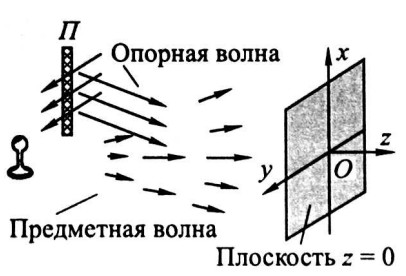
\includegraphics[width=0.5\textwidth]{pictures/hologram_recording.png}
    \caption{Схема записи голограммы}
    \label{fig:hologram_recording}
\end{figure}

При восстановлении изображения голограмма освещается опорной волной, и в результате дифракции света формируются три волны:
\begin{itemize}
    \item нулевой порядок дифракции — прошедший без изменений свет;
    \item волна, формирующая мнимое изображение объекта;
    \item волна, формирующая действительное изображение объекта.
\end{itemize}

\subsubsection{Голограмма точечного источника}

Для понимания принципов голографии рассмотрим простейший случай — голограмму точечного источника. При освещении такой голограммы плоской волной возникает три компоненты: прошедшая плоская волна, расходящаяся сферическая волна (формирует мнимое изображение) и сходящаяся сферическая волна (формирует действительное изображение).

\begin{figure}[h!]
    \centering
    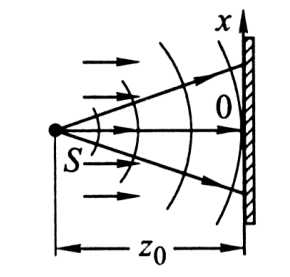
\includegraphics[width=0.4\textwidth]{pictures/point_source_hologram.png}
    \caption{Схема восстановления изображения с голограммы}
    \label{fig:point_source_hologram}
\end{figure}

Голограмма точечного источника имеет вид системы концентрических колец (зонная решётка Габора). Радиусы этих колец связаны с расстоянием $d$ от точечного источника до голограммы соотношением:
\begin{equation}
    \rho_m = \sqrt{m\lambda d},
    \label{eq:radius}
\end{equation}
где $m$ — номер кольца, $\lambda$ — длина волны, $\rho_m$ — радиус $m$-го кольца.

\subsubsection{Экспериментальная установка}

В работе исследуются голограммы точечного источника и трёхмерного объекта. Эти голограммы записаны на фотопластинках ЛОИ-2, имеющих высокое разрешение: $\approx 5000$ линий/мм. При записи был использован гелий-неоновый лазер с длиной волны излучения $\lambda = 532$ нм.

В работе требуется определить расстояние $d$ между голограммой и точечным источником света. Это расстояние можно рассчитать по формуле \eqref{eq:radius} из раздела 3.1, если измерить радиусы $\rho_m$ нескольких колец.

Для наблюдения голограммы используется установка, показанная на рис.~\ref{fig:scheme}. Голограмма Г освещается лазерным светом и формирует изображение на экране Э. Поскольку радиусы колец на исходной голограмме слишком малы для прямых измерений, используется увеличивающая линза Л.

\begin{figure}[h!]
    \centering
    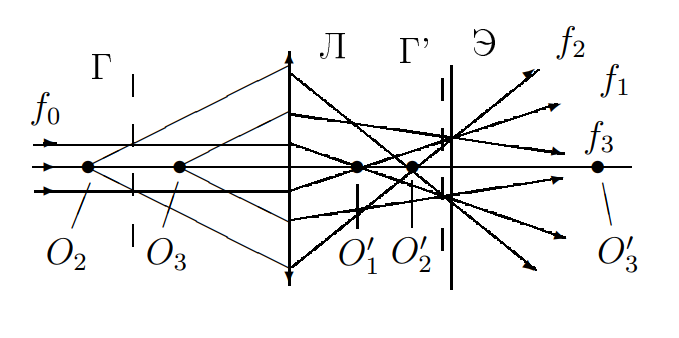
\includegraphics[width=0.7\textwidth]{pictures/scheme.png}
    \caption{Схема экспериментальной установки}
    \label{fig:scheme}
\end{figure}

Кроме голограммы точечного источника в работе исследуется голограмма объёмного предмета. При наблюдении такой голограммы можно увидеть эффект параллакса — изменение видимого положения элементов изображения при изменении угла наблюдения, что подтверждает объемный характер восстановленного изображения.

